\documentclass{article}

% \usepackage[margin=1in,includefoot]{geometry}
\usepackage{graphicx}
\usepackage{titlesec}
\usepackage[table]{xcolor}
\usepackage{color, colortbl}
\usepackage{stackengine}
\usepackage{fancyhdr}
\usepackage{longtable}
\usepackage{changepage}

\newcommand\xrowht[2][0]
{\addstackgap[.5\dimexpr#2\relax]{\vphantom{#1}}}
% \newcolumntype{C}{>{\centering\arraybackslash}p{0.6cm}}
% \newcolumntype{D}{>{\centering\arraybackslash}p{10cm}}
% \setlength{\parskip}{1em}

\setlength{\arrayrulewidth}{0.4mm}
\setlength{\tabcolsep}{20pt}
\renewcommand{\arraystretch}{1.6}
\setcounter{tocdepth}{4}
\setcounter{secnumdepth}{4}

\pagestyle{fancy}
\renewcommand{\headrulewidth}{2pt}
\renewcommand{\footrulewidth}{1pt}

\begin{document}
\begin{titlepage}
	\begin{center}
		\begin{figure}
			\centering
			
\includegraphics[scale=0.3]{LogoPolimi.PNG} \\
			[0.3cm]
		\end{figure}
		\Huge{\bfseries - RASD -} \\
		[0.5cm]
		\huge{Requirements Analysis and
			
			Specification Document} \\
		[1mm]
		\rule{300pt}{3pt} \\
		[1.0cm]
		\textsc{\Large Computer Science and Engineering} \\ 
		\textsc{\Huge Software Engineering II} \\
		\textsc{\Large A.A. 2020/2021} \\
		[1cm]
		\textsc{\LARGE Daniele Mammone - 10625264} \\
		\textsc{\LARGE Gianmarco Naro - 10610374} \\
		\textsc{\LARGE Massimo Parisi - 10583470} \\
	\end{center}
\end{titlepage}

\newpage
	
	\renewcommand\contentsname{Contents}
	\tableofcontents
	
\newpage

\section{Introduction}

	\subsection{Purpose}
	
	The main target of this document is to describe the software through functional and non-functional requirement and is used as contractual basis between the customer and the developer. The structure of the document follows the one studied during lectures and aim to describe faithfully the software behaviour in all of its aspects.
	
	The software in question is \emph{CLup}, a mobile service usable through app, made both for store managers and customers. It facilitates customers to book a visit to a store and, on the other hand, to help store managers to observe the new strict rules due to \emph{Covid-19}.
	
	\subsection{Scope}
	
	The main purpose of \emph{CLup} is to facilitate customers to access at a store in {\bfseries security}, both allowing them to reserve a spot on the queue for entering the store through the app and to book a visit at the store in a determined time window, selected by the user. Thanks to this, store managers can manage the {\bfseries affluency} in their store more easilier, and moreover can reduce the crowd in front of the store, that is the main purpose of the application. The main idea is that when a person's number is called, he can enter the supermarket. Moreover, the app should generate a \emph{QR Code} that the customer will scan at the entry and at the exit of the store, so that the system knows in real time how many people there are in the store. \emph{CLup} should also estimates the \emph{ETA} from the turn of a person. Moreover, it is able to suggest people other store options when there is a high waiting time to enter to the store requested by the user. The app also allows people to reserve their spot at the supermarket and, in order to optimize the waiting time, people can select specifics reparts where they want to go in the store.
	
	Summing up, \emph{CLup} has this main functionalities:
	
	\smallskip
	
	\begin{itemize}
		
		\item {\bfseries Manage of lining up of the store}: the app will manage the accesses to the store, based on numbered tickets released to people. When it's the turn of a person, it will be authorized to enter the shop. Futhermore, the store manager is able to manage the access and the affluency to the store.
		
		\item {\bfseries Booking visit}: users can book a visit at the store, in a certain time frame decided in the booking process. For them, there is no requirement of ticket, since are able to access the store only scanning the \emph{QR Code} at the store entrance. The system will grant access if the time of entering is correct.
		
		\item {\bfseries Alternatives}: the app is able to suggest other stores options and time if some store is full, or comfortable times aren't available at the moment of the booking.
	
	\end{itemize}

	%Following this brief introduction of the application scope, there are %the Phenomenon involved in the system.
		
		\subsubsection{World Phenomena}
		
		\bigskip
		
		\begin{center}
			
			\rowcolors{2}{}{gray!20}
			\rowcolors{1}{gray!20}{white}
			\renewcommand{\arraystretch}{2.5}
		
			\begin{adjustwidth}{-1.5cm}{}
			\begin{tabular}[h!]{|m{2.5em}|m{32.5em}|}
				
				\hline
				\xrowht{5pt}
				WP1 & A user enters a supermarket \\
				\xrowht{5pt}
				WP2 & A user waits in a lineup \\
				\xrowht{5pt}
				WP3 & A user exits the supermarket \\
				\xrowht{5pt}
				WP4 & A certain number of people is inside the supermarket \\
				\xrowht{5pt}
				WP5 & A certain number of people is at a specific repart of the supermarket \\
				\hline
			\end{tabular}
			\end{adjustwidth}
		
		\end{center}
	
		\smallskip
		
		\subsubsection{Shared Phenomena}
		
		\bigskip
		
		\begin{center}
			
			\rowcolors{2}{}{gray!20}
			\rowcolors{1}{gray!20}{white}
			\renewcommand{\arraystretch}{2.5}
			
			\begin{adjustwidth}{-1.5cm}{}
			\begin{tabular}[h!]{|m{2.5em}|m{27.5em}|m{1em}|}
				
				\hline
				\xrowht{5pt}
				SP1 & The user gets a ticket/QR & M\\
				\xrowht{5pt}
				SP2 & The user books a visit to the store & M\\
				\xrowht{5pt}
				SP3 & The store generates in presence a ticket & M\\
				\xrowht{5pt}
				SP4 & The user comes to knows how much time they have to wait before entering & U\\
				\xrowht{5pt}
				SP5 & The users know how many people there are in a store at a certain moment & U\\
				\xrowht{5pt}
				SP6 & The user scan the QR code and enters in the supermarket & U\\
				\xrowht{5pt}
				SP7 & The user scan the QR code and exits from the supermarket & U\\
				\xrowht{5pt}
				SP8 & The user can indicate the categories of items that he intend to buy & U\\
				\hline
				
			\end{tabular}
			\end{adjustwidth}
		
		\end{center}
		
		\subsubsection{Goals}
		
		\bigskip
		
		\begin{center}
			
			\rowcolors{2}{}{gray!20}
			\rowcolors{1}{gray!20}{white}
			\renewcommand{\arraystretch}{2}
			
			\begin{adjustwidth}{-1.5cm}{}
			\begin{tabular}[h!]{|m{2.5em}|m{32.5em}|}
				
				\hline
				\xrowht{5pt}
				G1 & Allow customers to select a store and book a spot on the queue from \emph{CLup} app \\
				\xrowht{5pt}
				G2 & Allow customers to book a spot on the queue from a physical ticket dispenser \\
				\xrowht{5pt}
				G3 & Allow store managers to regulate the influx of people in the building \\
				\xrowht{5pt}
				G4 & Allow people to select a better store option to avoid waisting a lot of time waiting to entry at a specific store. \\
				\xrowht{5pt}
				G5 & Allow users to depart from their location in time to avoid waiting too much, and to avoid losing their turn in lineup \\
				\xrowht{5pt}
				G6 & Allow users to decrease waiting times specifing reparts they want to visit \\
				\hline
				
			\end{tabular}
			\end{adjustwidth}
		\end{center}
	
		\bigskip
		
	\subsection{Definitions, Acronyms, Abbreviations}
	
		\smallskip
		
		\subsubsection{Definitions}
		
		\bigskip
		
		\begin{center}
			
			\rowcolors{2}{}{gray!20}
			\rowcolors{1}{gray!20}{white}
			\renewcommand{\arraystretch}{2}
			
			\begin{adjustwidth}{-1.5cm}{}
			\begin{tabular}[h!]{|m{8em}|m{27em}|}
				
				
				\hline
				\xrowht{5pt}
				QR Code & Bidimensional bar code that allows the user to check-in/check-out \\
				\xrowht{5pt}
				Customer & The clients of the store, that uses the application part reserved to bookings \\
				\xrowht{5pt}
				Store manager & The user that access to stores' bookings and occupancy, in order to manage the flow of customers \\
				\xrowht{5pt}
				QR Code Reader & Device used to scan customers' QR Code \\
				\xrowht{5pt}
				Totem & Electronic device that allows customers to book a store visit, allowing them to specifiy the same parameters that can be inserted through the app \\
				\xrowht{5pt}				
				QR Code Printer & Device used to print QR Code at the stores \\
				\xrowht{5pt}
				Repart & Part of the store that contains the same category of products \\
				\hline
			\end{tabular}
			\end{adjustwidth}
			
		\end{center}
	
		\smallskip
		
		\subsubsection{Acronyms}
		
		\bigskip
		
		\begin{center}
			
			\rowcolors{2}{}{gray!20}
			\rowcolors{1}{gray!20}{white}
			
			\begin{adjustwidth}{-1.5cm}{}
			\begin{tabular}[h!]{|m{3.5em}|m{31.5em}|}
				
				\hline
				\xrowht{5pt}
				RASD & Requirement Analysis and Specification Document \\
				\xrowht{5pt}
				ETA & Estimated Time of Arrival \\
				\xrowht{5pt}
				GPS & Global Positioning System \\
				\hline
				
			\end{tabular}
			\end{adjustwidth}
			
		\end{center}
	
		\bigskip
		
		\subsubsection{Abbreviations}
		
		\bigskip
		
		\begin{center}
			
			\rowcolors{2}{}{gray!20}
			\rowcolors{1}{gray!20}{white}
			
			\begin{adjustwidth}{-1.5cm}{}
			\begin{tabular}[h!]{|m{2.5em}|m{32.5em}|}
				
				\hline
				\xrowht{5pt}
				WPn & World phenomena number n \\
				\xrowht{5pt}
				SPn & Shared phenomena number n \\
				\xrowht{5pt}
				Gn & Goal number n \\
				\xrowht{5pt}
				Rn & Requirement number n \\
				\hline
				
			\end{tabular}
			\end{adjustwidth}
		\end{center}
	
		\smallskip
		
	\subsection{Revision History}
	
	\bigskip
	
	\begin{center}
		
		\begin{adjustwidth}{-1.5cm}{}
		\begin{tabular}[h!]{|m{4em}|m{5em}|m{22em}|}
			
			\hline
			\rowcolor{gray!20}
			\xrowht{5pt}
			Version & Date & Changelog \\
			\hline
			\xrowht{5pt}
			1.0 & 10/11/2020 & Overview of the specifications and initial draft of the document \\
			\hline
			
		\end{tabular}
		\end{adjustwidth}
		
	\end{center}

	\bigskip

	\subsection{Reference Documents}
	
		\smallskip
		
		\begin{itemize}
			
			\item Specification Document
			\item Slides of the lectures
			
		\end{itemize}
	
	\newpage 
	
	\subsection{Document Structure}
	
	The structure of the document is thought with the intention of allowing simple navigation throght it. Also, various abbreviations, highlighted in Abbreviations section, have been used to make the content smoother.
	Hence, the structure of the document is the following one:
	
	\begin{itemize}
		
		\item {\bfseries Introduction}: The main purpose of this section is to introduce in a general way the scope of the application throght the analysis of the \emph{World Phenomena}, \emph{Shared Phenomena} and \emph{Goals}. Moreover, the main functions of the software are illustrated and the abbreviations, acronyms and definitions are defined in order to allow an easy reading.
		
		\item {\bfseries Overall Description}: The section starts with a summary description of the UML of the software, so as to have a general presentation of the operation of the application. Then, in order to clarify the behaviour of the application, there are state charts of the most important functions and the detailed description of all software functions. Subsequently, the section ends with the most important phenomena that cannot be managed by the system.
		
		\item {\bfseries Specific Requirements}: The main focus of this section is to describe the essential hardware and software interfaces and requirements, indeed \emph{CLup} uses this interfaces to provide its services to the external world. After this, there is the core of the section represented by use cases that provides detailed information about the relation with requirements.
		
		\item {\bfseries Formal Analysis Using Alloy}: This section describes formally the model using Alloy language, highlighting the main problems of the software, solving them in a formal way.
		
		\item {\bfseries Effort Spent}: The main focus of this section is to track the time spent to complete this project. In particular, is highlighted the subdivision of the working hours of the various sections
		
		\item {\bfseries References}: This section is dedicated to all refercences used in this project.
		
	\end{itemize}
	
\newpage	

\section{Overall Description}

	\subsection{Product Perspective}
	
	In Figure ??? is reported an UML Class Diagram that represents the domain of the application with main concepts and data involved, including their relationships.
	
	The store managers registers to the application providing all necessary information and can decide at a later stage to modify the capability options (regarding each department of the store). The customer simply downloads the application on his device to be able to use it. Here we can identify the main aspects related to CLup:
	
	\begin{itemize}
		
		\item The customer can generate a reservation, choosing between the registered chain store (and one of their specific store) or a normal store, a time slot and, optionally, the departments that they want to access; CLup will retrieve a ticket containing the number of the reservation and a QR code.
		
		\item The customer can entry in the store where he has a reservation (on the right time slot) scanning the QR code with a totem/the help of a store manager.
		
		\item The customer exit the store reusing the QR code, notifying the application that a new spot in now free (on certain department).
		
	\end{itemize}
	
	The UML does not include every class of the actual implementation of the system.
	
		\subsubsection{UML Description}

		{\bfseries Inserire UML qui}
		
		\subsubsection{State Charts}
		
		Now we are going to examine some essential aspects of the application, modelling their behaviours and showing the evolutin over time of their states through adequate state diagrams, which are reported below.
		
		\begin{figure}[!h]
			
			\centering
			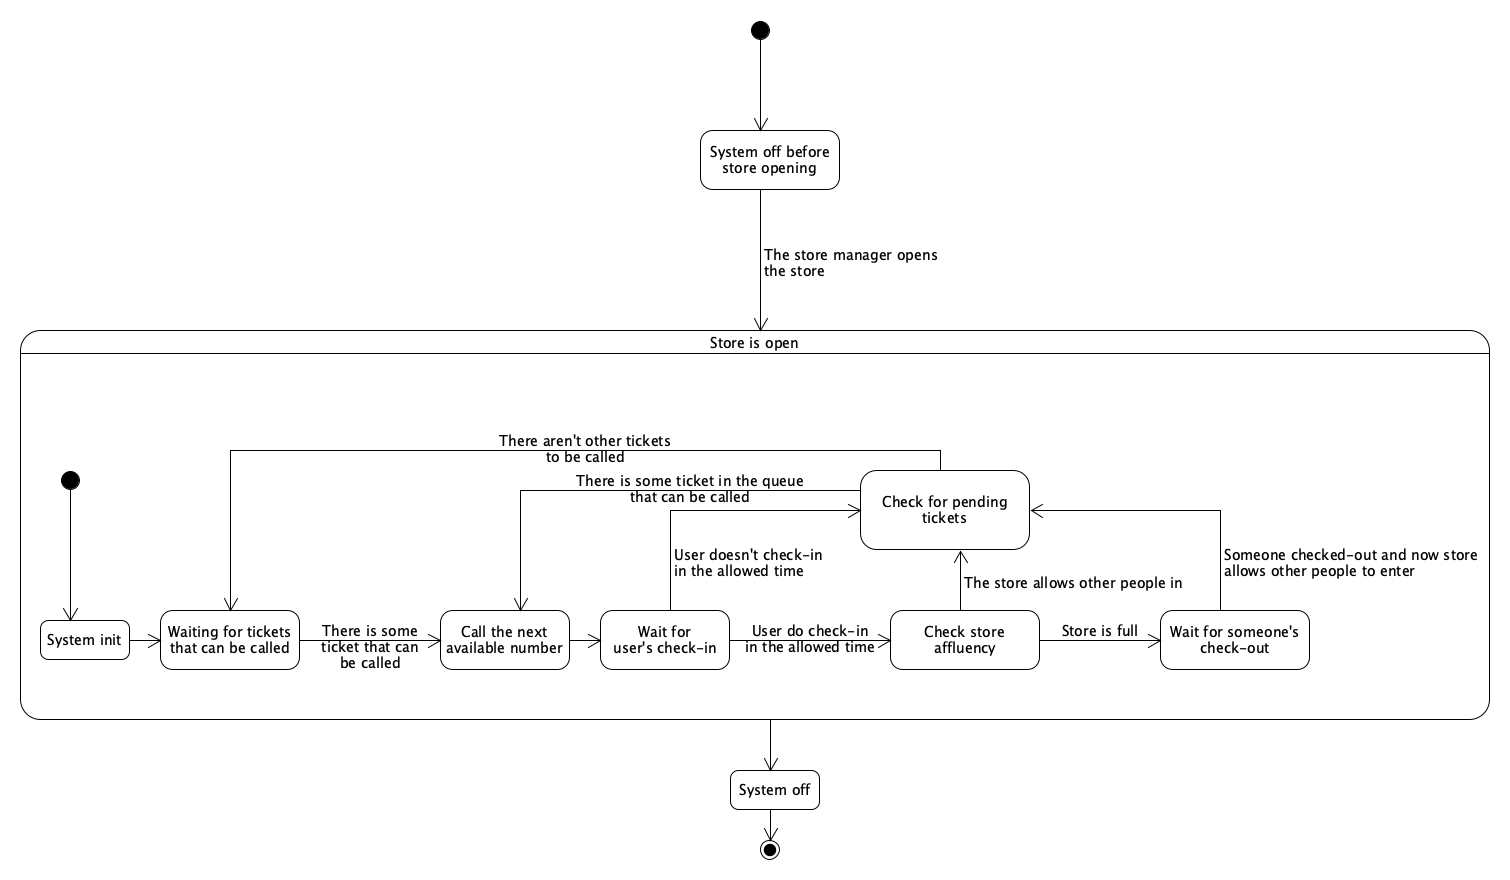
\includegraphics[scale=0.23]{statechart1.PNG} \\
			\caption{Number calling system}
			
		\end{figure}
	
		When the store manager opens the store, the system initialize itself and waits for some ticket that can be called. For example, tickets related to the \emph{FIFO} queue can be called as soon as the requested zones are available, and tickets related to bookings can be called only after the start time of the booked time slot, and will be called around this time, when all the booked zones become available (to avoid starvation on calling bookings, other tickets requesting at least one booked zone won't be called until the booked tickets enters the supermarket). After a ticket is available to be called, the system notify in some way (e.g. through a store employee) that now certain ticket is allowed to enter the store. At this point, the system waits for the scan of the associated \emph{QR code}. If the customer doesn't check-in in the assigned time, the system discard the ticket and checks if there are other available tickets. If so, it return in the state of calling the number; else, it will wait for an eligible ticket to be called. If the user, otherwise, scan his \emph{QR code} in time, the system checks the affluence of the store. If it's full, the system will wait for someone's check out, in order to check if some ticket can be called. Else, if the store isn't full, the system doesn't have to wait for a check out to check if there is some ticket eligible to be called. When at some time the store manager will close the store, the system begins its shutdown procedure. It's assumed that at the closure there isn't any other uncalled ticket, since at a certain point the generation of tickets will be blocked, so that that the last ticket will be served around the time of closure.
		
		\bigskip
		
		\begin{figure}[!h]
			
			\centering
			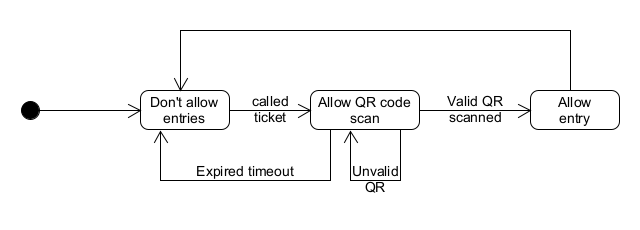
\includegraphics[scale=0.52]{statechart2.PNG} \\
			\caption{QR Code scanner state machine}
			
		\end{figure}
		
		The system doesn't allow entries since a ticket is called by the system described above. Than, the QR code reader waits for a QR code to be scanned. When a QR is scanned, the system checks if it's a valid one; if so, allows the entry, otherwise notify the wrong QR code and continue waiting for the right one. If the valid QR isn't scanned in time, the system block the entry and waits for the next called ticket. Otherwise, if the valid QR code is scanned in time, the system allows the entry and, detected the entry, or expired the timeout, block the entries and waits for the next ticket to be called.
	
	\subsection{Product Functions}
		
	In the previous chapter there were introduced, sketchily, the main features of the software in order to understand, in general, its functioning. Alternatively, in this section will be illustrated and described accurately all the functions that the software allows to do.
	
		\subsubsection{Getting a ticket}
		
		In order to manage the line of the supermarket, it's used a system based on the "call of numbers". Each user in the queque has a unique ID, and when his number is called (eg. by a store employee), the user is authorized to enter. This mechanism works also for the booking feature, since the system generates a number that won't be called until the beginning of the time slot selected by the user. Users can get a ticket both on the application and at a totem installed at the entry of the store (obviously, on the app users are required to select some specific store of their preference from a given list, sorted by the nearest one from the position obtained from the \emph{GPS}). With the generation of the ticket, the user will get both an ID and a \emph{QR Code} associate to it, to be scanned at the enter of the store. When getting a ticket on the application, users must be logged in with their credentials (if not, they must register at the services following the procedure that will be explained later), while at the Totem they can simply get the ticket without giving any data. On app, customers get a digital ticket with its associated \emph{QR Code}; at totem, the ticket and the qr code will be printed. On both of them, there is displayed the expeted time of call. Getting the ticket, the user can indicate the repart in which he is interested, and using the app can decide both to have a ticket to enter asap in the store or to plan his visit. At the store's totem, he can only get a ticket to enter as soon as possible. Once completed the operation on the app, the user will be able to see at any moment the time needed to reach the store by the preferred mean of transport selected in the settings.
		
		\subsubsection{Calling process}
		
		The process to admit people in the store follows a \emph{FIFO} logic: the first one that got a ticket, is the first to access the store. When called, a person is authorized to access the store. To register his entry, he is requested to check-in at the entry in a certain amount of time. \\
		
		\subsubsection{Check-in/Check-out}
		
		At the store entries and exities, users have to scan their \emph{QR Codes} to respectively Check-in and Check-Out in the supermarket. If someones doesn't check-in in a prefixed amount of time, definible by the store manager, he'll lost his turn in the queue. \emph{QR Code} scan is required for two important reasons: register someone's entry in the store for contact tracing purposed, and to check that the person entering the store is the one called, to avoid stoles of turns. \\
		
		\subsubsection{Plan a visit}
		
		The app allows to brand's customers to plan a visit in a store of their preference. At the end of the process of getting a ticket, if the user select to plan his visit to the store, the software shows the user the time table highlighting the days and the time slots available, in such a way as to allow the user to select the best option for him. If the options do not satisfy the user, he can ask the application for help to find other supermarkets with more comfortable hours. If a reservation process is interrupted in the middle, the user will be able to resume it reopening the app. \\
		
		\subsubsection{Managing single reparts}
		
		In the process of getting a ticket, users can indicate the categories of items that they intend to buy in the store, so that it's possible to optimize the waiting time, or they may skip the process, booking a visit to the whole store, but this may lead to greater waiting time, because they can enter the store only when all the reparts are free at the same time. In fact, each repart has a fixed capacity of admitted people, so that each prenotation in line can be called when each selected repart is available. It's obvious that selecting the whole store option, the waiting times are greater. \\
		
		\subsubsection{Notify users}
		
		If some account have non completed visits, depending on the position of the client (retrieved by \emph{GPS}), and the preferred option of reaching the selected store (eg. on foot, by car or public transport), the app will notify the client when he can exit home, to arrive in time to enter the supermarket, without losing its turn and avoiding long waiting times. Notice that not all of the moving options may be available in all the places, since it depends on the used map service. \\
		
		\subsubsection{Cancel a visit}
		
		If the user can not reach the store in time, he can decide to cancel the booked visit or the generated ticket. In this case the software delete the customer from the queue and rearrange the last one. \\
		
		\subsubsection{Store capacity}
		
		The app, also, allows store managers to see the store's affluency and to modify the store capacity in every single repart. When a repart capacity is changed, the latest overflowing bookings will be cancelled, and a notify is sent to the customer, proposing him other comfortable options for the same preferences. \\
		
		\subsubsection{Infer waiting time from users}
		
		The system can infer the average time spent by a user in the supermarket using the previous visits as data. When a user get a ticket for the first time without planning his visit, he's asked to enter a reasonable time that he will spend in the supermarket. For the next visits, app will infer this time by time spent in store between check in and check out, so that can estimate more accurately waiting times, and to suggest users better time options while planning their visit. \\

	\subsection{User Characteristics}
	
	\emph{CLup} gives access to two different sets of functionalities based on the two different category of users:
	
	\begin{itemize}
		
		\item {\bfseries Customer}: Allows user to book a visit to the supermarket. The software generates a \emph{QR Code} that the user can use to enter in the supermarket. The user can indicate the exact list of items that he intends to purchase, or, at least, the categories of items that he intends to buy and, also, he can indicates the approximate expected duration of the visit. Moreover, the user can see the \emph{ETA} to enter the store. \emph{CLup} also allows clients to obtain their book at the store entry.\\
		
		\item {\bfseries Store Manager}: The Store Manager can view information about the store, in particular he can access to the reservations made by users to predict the future affluency and check the level of affluency in the store (and also in specific zones of the store) \\
		
	\end{itemize}

	\subsection{Assumptions, Dependencies, Constraints}
	
		\subsubsection{Domain Assumptions}
		
		extra


\section{Specific Requirements}
	\subsection{External Interface Requirements}
		\subsubsection{User Interfaces}
		\subsubsection{Hardware Interfaces}
		\subsubsection{Software Interfaces}
		\subsubsection{Communication Interfaces}
	\subsection{Functional Requirements}
		\subsubsection{List of Requirements}
		extra
		\subsubsection{Mapping}
		extra
		\subsubsection{Use Cases}
		
			\newpage
			
			\paragraph{Registration of a customer}
			
				\begin{center}
					
					\rowcolors{2}{}{gray!20}
					\rowcolors{1}{gray!20}{white}
					
					\begin{adjustwidth}{-1.5cm}{}
					\begin{tabular}[h!]{|m{7.5em}|m{27.5em}|}
						
						\hline
						\xrowht{5pt}
						Name &  Registration of a customer\\
						\xrowht{5pt}
						Actors & Customer\\
						\xrowht{5pt}
						Entry Condition & Customer has the internet connection available and has accessed the application on its device\\
						\xrowht{5pt}
						Event Flow & \begin{enumerate}
							
							\itemsep-0.25em
							\item Customer visualizes the initial page of the app
							\item Customer clicks on “Sign up as customer” button
							\item Customer inserts a username, a password, an e-mail, his name, his surname and his phone number as mandatory fields
							\item The system confirms the registration of the customer
							\item The system saves the information of the customer
							
						\end{enumerate}\\
						\xrowht{5pt}
						Exit Conditions & Customer is successfully registered to the application\\
						\xrowht{5pt}
						Exception & \begin{enumerate}
							
							\itemsep-0.25em
							\item The username is already present in the system
							\item The customer did not fill up all the mandatory fields with valid data
						
						\end{enumerate}
						If one or more of the above situations occur, the application will throw an error message and will return to the registration form page\\		
						\hline
						
					\end{tabular}
					\end{adjustwidth}
					
				\end{center}
		
			\paragraph{Registration of a store}
			
				\begin{center}
					
					\rowcolors{2}{}{gray!20}
					\rowcolors{1}{gray!20}{white}
					
					\begin{adjustwidth}{-1.5cm}{}
					\begin{tabular}[h!]{|m{7.5em}|m{27.5em}|}
						
						\hline
						\xrowht{5pt}
						Name & Registration of a store\\
						\xrowht{5pt}
						Actors & Store manager\\
						\xrowht{5pt}
						Entry Condition & Store manager has the internet connection available and has accessed the application on its device\\
						\xrowht{5pt}
						Event Flow & \begin{enumerate}
							
							\itemsep-0.25em
							\item Store manager visualizes the initial page of the app
							\item Store manager clicks on “Sign up as store” button
							\item Store manager compile all the mandatory fields concerning the store
							\item Store manager loads a certification document which proves that it is a real store
							\item The system validates the certification
							\item The system confirms the registration of the store
							\item The system saves the information of the store
							
						\end{enumerate}\\
						\xrowht{5pt}
						Exit Conditions & The store is successfully registered to the application\\
						\xrowht{5pt}
						Exception & \begin{enumerate}
							
							\itemsep-0.25em
							\item The store is already present in the system
							\item The store manager did not fill up all the mandatory fields with valid data
							\item The certification is invalid
							
						\end{enumerate}
						If one or more of the above situations occur, the application will throw an error message and will return to the registration form page\\		
						\hline
						
					\end{tabular}
					\end{adjustwidth}
					
				\end{center}
		
			\paragraph{Login of a customer}
			
				\begin{center}
					
					\rowcolors{2}{}{gray!20}
					\rowcolors{1}{gray!20}{white}
					
					\begin{adjustwidth}{-1.5cm}{}
					\begin{tabular}[h!]{|m{7.5em}|m{27.5em}|}
						
						\hline
						\xrowht{5pt}
						Name & Login of a customer\\
						\xrowht{5pt}
						Actors & Customer\\
						\xrowht{5pt}
						Entry Condition & Customer is already registered to the application service\\
						\xrowht{5pt}
						Event Flow & \begin{enumerate}
							
							\itemsep-0.25em
							\item Customer accesses the application through its device
							\item Customer clicks on “Login as customer” button
							\item The system opens the “Login as customer” page
							\item Customer compiles the fields “Username” and “Password”
							\item Customer clicks on “Login” button
							\item The system opens the “Customer menu” page
							
						\end{enumerate}\\
						\xrowht{5pt}
						Exit Conditions & Customer has successfully logged in\\
						\xrowht{5pt}
						Exception & \begin{enumerate}
							
							\itemsep0em
							\item Customer enters invalid Username
							\item Customer enters invalid Password
							
						\end{enumerate}
						If one or more of the above situations occur, the application will throw an error message and will return to the “Login as customer” page\\		
						\hline
						
					\end{tabular}
					\end{adjustwidth}
					
				\end{center}
			
			\paragraph{Login of a store manager}
			
				\begin{center}
					
					\rowcolors{2}{}{gray!20}
					\rowcolors{1}{gray!20}{white}
					
					\begin{adjustwidth}{-1.5cm}{}
					\begin{tabular}[h!]{|m{7.5em}|m{27.5em}|}
						
						\hline
						\xrowht{5pt}
						Name & Login of a store manager\\
						\xrowht{5pt}
						Actors & Store manager\\
						\xrowht{5pt}
						Entry Condition & Store manager’s store is already registered to the application service\\
						\xrowht{5pt}
						Event Flow & \begin{enumerate}
							
							\itemsep-0.25em
							\item Store manager accesses the application through its device
							\item Store manager clicks on “Login as store” button
							\item The system opens the “Login as store” page
							\item Store manager compiles the fields “ID” and “Password”
							\item Store manager clicks on “Login” button
							\item The system opens the “Store menu” page
							
						\end{enumerate}\\
						\xrowht{5pt}
						Exit Conditions & Store manager has successfully logged in\\
						\xrowht{5pt}
						Exception & \begin{enumerate}
							
							\itemsep-0.25em
							\item Store manager enters invalid ID
							\item Store manager enters invalid Password
							
						\end{enumerate}
						If one or more of the above situations occur, the application will throw an error message and will return to the “Login as store” page\\		
						\hline
						
					\end{tabular}
					\end{adjustwidth}
					
				\end{center}
			
			\paragraph{Customer makes a reservation}
			
				\begin{center}
					
					\rowcolors{2}{}{gray!20}
					\rowcolors{1}{gray!20}{white}
					
					\begin{adjustwidth}{-1.5cm}{}
					\begin{tabular}[h!]{|m{7.5em}|m{27.5em}|}
						
						\hline
						\xrowht{5pt}
						Name & Customer makes a reservation\\
						\xrowht{5pt}
						Actors & Customer\\
						\xrowht{5pt}
						Entry Condition & Customer is already logged in the application service\\
						\xrowht{5pt}
						Event Flow & \begin{enumerate}
							
							\itemsep-0.25em
							\item Customer clicks on “Make a reservation”
							\item The system opens the “Reservation” page
							\item The customer can see the list of stores in his city and can filter this list by choosing a specific chain from a drop down menu
							\item Customer selects a store and clicks on “Next” button
							\item The system opens the “Objects’ category” page
							\item Customer can see the list of all possible objects’ category and can select some of them (optional)
							\item Customer click on “Next” button to confirm the selection
							\item The system opens the “Time preference” page
							\item Customer can see two button, “As soon as possible” and “Choose a time slot”
							 
							\begin{enumerate}
								
								\itemsep-0.25em
								\item if the customer clicks on “As soon as possible” button, the system will check if there is a free spot on the following hour
								
								\begin{enumerate}
									
									\itemsep0em
									\item if there is a free spot, the system will generate a
									QR code, show it to the customer and save it in the
									database
									\item otherwise, the system will inform the customer and suggest him stores less crowded
									
								\end{enumerate}
								
								\item if the customer clicks on “Choose a time slot”, the system will open the “Time slots” page, where he can see all the available time slot, and clicking on one of them will generate a QR code, that will be showed to the customer and saved in the database
								
							\end{enumerate}
							
						\end{enumerate}\\
						\xrowht{5pt}
						Exit Conditions & Customer has successfully made a reservation\\
						\xrowht{5pt}
						Exception & \begin{enumerate}
							
							\itemsep-0.25em
							\item Customer click on a timeslot no longer available
							\item Customer tries to book more than the set limit of reservations per week
							
							If the above situation occur, the application will throw an error message and will reload the “Time slots” page (updating it)
							
							\item Customer doesn’t select any product category
							
							If the above situation occurs, the application will throw an error and ask the client to select at least some item.
							
							\item Customer tries to get a ticket while he already have a unused one 
							
						\end{enumerate}
						If the above situation occurs, the application shows an error message and invite the client to use the pending ticket\\		
						\hline
						
					\end{tabular}
					\end{adjustwidth}
					
				\end{center}
			
			\paragraph{Customer visualizes reservations}
			
				\begin{center}
					
					\rowcolors{2}{}{gray!20}
					\rowcolors{1}{gray!20}{white}
					
					\begin{adjustwidth}{-1.5cm}{}
					\begin{tabular}[h!]{|m{7.5em}|m{27.5em}|}
						
						\hline
						\xrowht{5pt}
						Name & Customer visualizes reservations\\
						\xrowht{5pt}
						Actors & Customer\\
						\xrowht{5pt}
						Entry Condition & Customer is already logged in the application service and made a reservation\\
						\xrowht{5pt}
						Event Flow & \begin{enumerate}
							
							\itemsep-0.25em
							\item Customer clicks on “Show requests” button
							\item The app show the list of bookings made and tickets requested
							\item The customer select the desired option
							\item The system opens the detail page of the selected option, that includes the “QR Code” and the number that should be called, among with the scheduled entry date and time
							
						\end{enumerate}\\
						\xrowht{5pt}
						Exit Conditions & Customer can visualize the QR code\\
						\xrowht{5pt}
						Exception & None\\	
						\hline
						
					\end{tabular}
					\end{adjustwidth}
					
				\end{center}
			
			\paragraph{Manager modifies store parameters}
			
				\begin{center}
					
					\rowcolors{2}{}{gray!20}
					\rowcolors{1}{gray!20}{white}
					
					\begin{adjustwidth}{-1.5cm}{}
					\begin{tabular}[h!]{|m{7.5em}|m{27.5em}|}
						
						\hline
						\xrowht{5pt}
						Name & Store manager modifies store parameters\\
						\xrowht{5pt}
						Actors & Store manager\\
						\xrowht{5pt}
						Entry Condition & Store manager is already logged in the application service\\
						\xrowht{5pt}
						Event Flow & \begin{enumerate}
							
							\itemsep-0.25em
							\item Store manager clicks on “Modify parameters” button
							\item The system opens the “Modify parameters” page
							\item Store manager can see the name of each parameter flanked by a modifiable text box containing the previous value of that parameter (eg. zone capacity, store capacity)
							
							\begin{enumerate}
								
								\itemsep0em
								\item Store manager modify one, more or none of the parameters and clicks “Save changes” button
								\item Store manager choose to add/delete (except for the default parameters “Store capacity” and “Maximum number of weekly reservations for client”) some parameter of the store
								
							\end{enumerate}
							\item The system save the changes and bring him back to “Store menu” page
							
						\end{enumerate}\\
						\xrowht{5pt}
						Exit Conditions & Store manager has successfully updated store parameters\\
						\xrowht{5pt}
						Exception & \begin{enumerate}
							
							\itemsep-0.25em
							\item Store managers enters an invalid value for one or more parameters
							\item The store manager tries to add an already existing parameter, or tries to delete the default “Store capacity” and “Maximum number of weekly reservations for client” parameters
							\item The sum of the capacities of the single zones is greater than the store capacity
							
						\end{enumerate}
					
						If the above situation occur, the application will throw an error message and will return to “Modify parameters” page\\	
						\hline
						
					\end{tabular}
					\end{adjustwidth}
					
				\end{center}
			
			\paragraph{The store manager monitors the store situation}
			
				\begin{center}
					
					\rowcolors{2}{}{gray!20}
					\rowcolors{1}{gray!20}{white}
					
					\begin{adjustwidth}{-1.5cm}{}
					\begin{tabular}[h!]{|m{7.5em}|m{27.5em}|}
						\hline
						\xrowht{5pt}
						Name & Store manager modifies store parameters\\
						\xrowht{5pt}
						Actors & Store manager\\
						\xrowht{5pt}
						Entry Condition & Store manager has opened the app and is already logged in\\
						\xrowht{5pt}
						Event Flow & \begin{enumerate}
							
							\itemsep-0.25em
							\item Manager clicks on “Monitor store” button
							\item The app shows a page with statistics on the store, including number of people inside the store, percentage of store occupation and the number of daily access to the building
							
							\begin{enumerate}
								\item If the manager wants, he can see the same statistics per store zone by clicking the “monitor zones” button. The system will show all the zones sorted by criticity
							\end{enumerate}
							
						\end{enumerate}\\
						\xrowht{5pt}
						Exit Conditions & Store manager can see statistics on the store\\
						\xrowht{5pt}
						Exception & None\\	
						\hline
						
					\end{tabular}
					\end{adjustwidth}
					
				\end{center}
			
			\paragraph{The store manager manages customers bookings}
			
				\begin{center}
					
					\rowcolors{2}{}{gray!20}
					\rowcolors{1}{gray!20}{white}
					
					\begin{adjustwidth}{-1.5cm}{}
						\begin{tabular}[h!]{|m{7.5em}|m{27.5em}|}
							\hline
							\xrowht{5pt}
							Name & The store manager manages customers bookings\\
							\xrowht{5pt}
							Actors & Store manager\\
							\xrowht{5pt}
							Entry Condition & Store manager has opened the app and is already logged in\\
							\xrowht{5pt}
							Event Flow & \begin{enumerate}
								
								\itemsep-0.25em
								\item Manager clicks on “Manage bookings” button
								\item The app shows a list of reservations, with some of their details in preview (such as chosen date and time slot)
								\item The manager can choose one of them, and the app will show some possibilities to the manager
								
								\begin{enumerate}
									
									\item The manager can press on the button “Contact client” to contact the client for some reasons.
									
									\begin{enumerate}
										
										\item The manager can choose to contact the client via mail clicking on the button “Email option”
										
										\begin{enumerate}
											
											\item The app will show an interface where the manager can insert the text
											\item The manger clicks on the “Send” button to send the message
											
										\end{enumerate}
									
										\item The manager can choose to call the client clicking on the “Call customer” button
										
										\begin{enumerate}
											
											\item The app will invoke mobile OS API to start a call
											
										\end{enumerate}
									
										\item The app returns to the previous page
										
										
									\end{enumerate}
								
									\item The manager can click on the button “Cancel booking” to cancel a reservation
									
									\begin{enumerate}
										
										\item The app will show a dialog box where the manager can put-in an optional message, explaining the reasons of the cancel
										\item The manager clicks on the “Delete button”
										\item The app will show a confirmation box to ask if the manager is sure to proceed
										\item The manager clicks on “Yes” to confirm the deletion
										\item The app closes the dialog box
										
									\end{enumerate}
								
									\item The manager can choose to reschedule a booking
									
									\begin{enumerate}
										
										\item The app will show a dialog box where the manager can choose a new time slot and insert a message explaining the reasons
										\item The manager clicks on “Modify” to modify the booking
										\item The app closes the dialog box
										
									\end{enumerate}
									
								\end{enumerate}
								
							\end{enumerate}\\
							\xrowht{5pt}
							Exit Conditions & Store manager can manage the store and is able to edit reservations\\
							\xrowht{5pt}
							Exception & None\\	
							\hline
							
						\end{tabular}
					\end{adjustwidth}
					
				\end{center}
			
			\paragraph{Customers reservations management}
			
				\begin{center}
					
					\rowcolors{2}{}{gray!20}
					\rowcolors{1}{gray!20}{white}
					
					\begin{adjustwidth}{-1.5cm}{}
						\begin{tabular}[h!]{|m{7.5em}|m{27.5em}|}
							\hline
							\xrowht{5pt}
							Name & Customers reservations management\\
							\xrowht{5pt}
							Actors & Customer\\
							\xrowht{5pt}
							Entry Condition & The customer has the application opened, is logged in and has at least one pending request\\
							\xrowht{5pt}
							Event Flow & \begin{enumerate}
								
								\itemsep-0.25em
								\item The user press on the “Show requests” button
								\item The app shows a page with the requests made by the client
								\item The user selects the desidered requests
								\item The app will show the requests details
								\item The user press the “edit” button
								
								\begin{enumerate}
									
									\item If the selected requests is a ticket, the customer can delete it pressing the “Delete button”
									
									\begin{enumerate}
										
										\item The system will show a confirmation dialogue
										\item The client press the yes button
										\item The ticket is deleted and the app will return to the previous screen if there are other requests, or to the main menu otherwise
										
									\end{enumerate}
								
									\item If the selected request is a booking, the client can both click the delete button, and follow the above procedure or can select the “modify button”
									
									\begin{enumerate}
										
										\item If the modify button is selected, the app will restart the “Make a reservation process” described in Use Case n. 5. The customer can modify all the parameters of his reservation, including transforming it in a “As soon as possible ticket
										 
									\end{enumerate}
									
								\end{enumerate}
								
							\end{enumerate}\\
							\xrowht{5pt}
							Exit Conditions & The client can modify his reservation\\
							\xrowht{5pt}
							Exception & None\\	
							\hline
							
						\end{tabular}
					\end{adjustwidth}
					
				\end{center}
			
		\subsubsection{Sequence Diagram}
		extra
		\subsubsection{Scenarios}
		extra
	\subsection{Performance Requirements}
	\subsection{Design Costraints}
		\subsubsection{Standards Compliance}
		\subsubsection{Hardware Limitations}
		\subsubsection{Any Other Constraint}
	\subsection{Software System Attributes}
		\subsubsection{Reliability}
		\subsubsection{Availability}
		\subsubsection{Security}
		\subsubsection{Maintainability}
		\subsubsection{Portability}
	\subsection{Additional Specifications}
	extra
	
	
\section{Formal Analysis Using Alloy}
	\subsection{Alloy}
	extra
	
	
\section{Effort Spent}

\section{References}	
	
	
	
\end{document}